%%%%%%%%%%%%%%%%%%%%%%%%%%%%%%%%%%%%%%%%%%%%%%%%%%%%%%%%%%%%%%%%%%%%%%%%%%%%%%%%%%
\begin{frame}[fragile]\frametitle{}
\begin{center}
{\Large Chain of Thought Reasoning}

{\tiny (Ref: Vizuara's Substack)}

\end{center}

\end{frame}


%%%%%%%%%%%%%%%%%%%%%%%%%%%%%%%%%%%%%%%%%%%%%%%%%%%%%%%%%%%
\begin{frame}[fragile]\frametitle{Introduction to Reasoning LLMs}

      \begin{itemize}
        \item GPT-3.5 (Dec 2022) was designed to answer like humans, not think like humans
        \item Evolution from basic response models to reasoning-capable LLMs
        \item OpenAI's O1 model was first reasoning-based model
        \item Deep reasoning capabilities emerged in models like DeepSeek
        \item Timeline: 2022 onwards marks serious reasoning LLM development
        \item Most LLM providers now have reasoning models in their arsenal
      \end{itemize}

        \begin{center}
        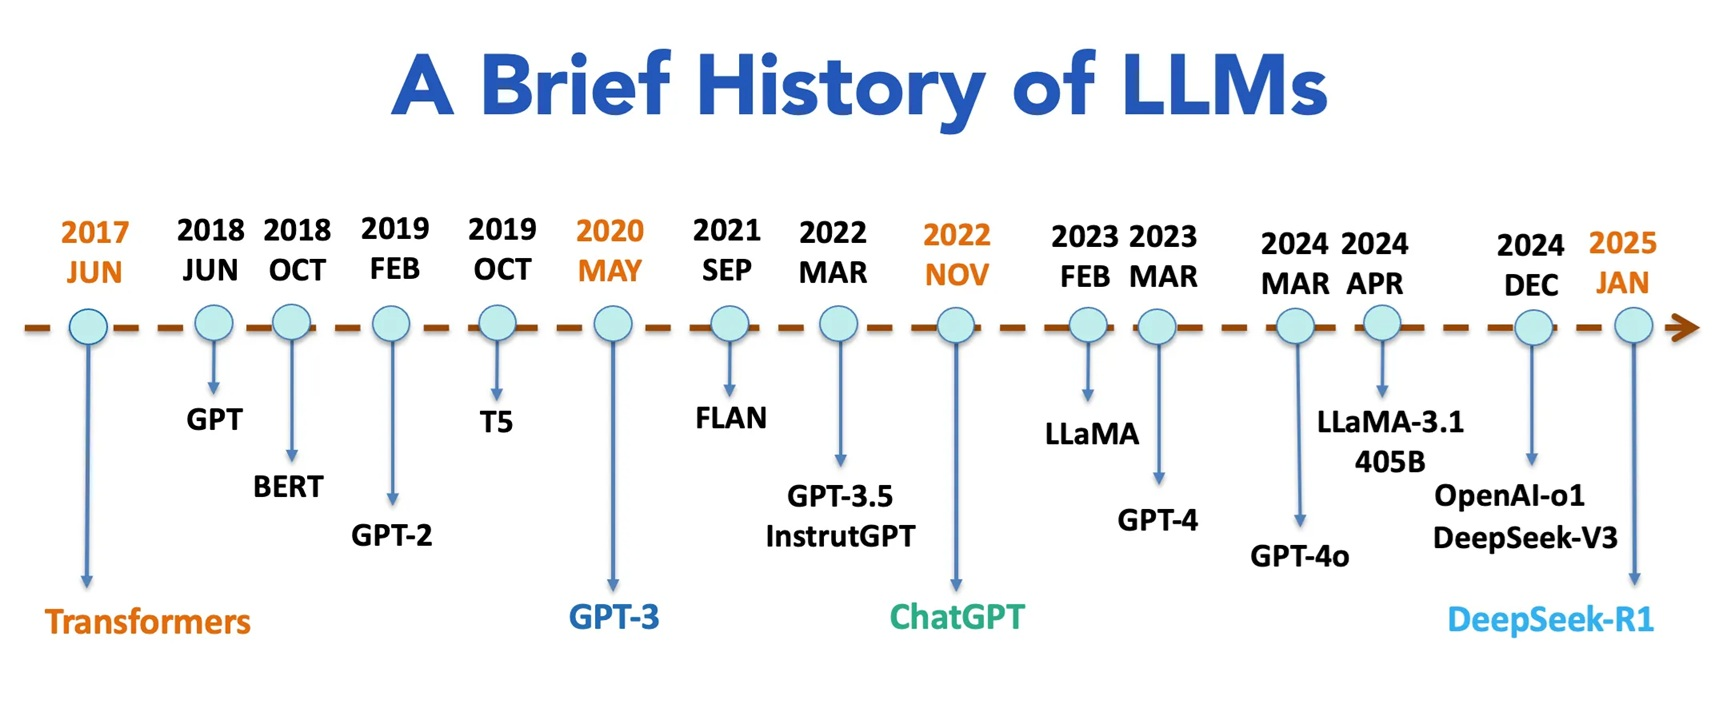
\includegraphics[width=0.8\linewidth,keepaspectratio]{llm211}
		
		{\tiny (Ref: A Brief History of LLMs - LM Pro)}

        \end{center}	

\end{frame}

%%%%%%%%%%%%%%%%%%%%%%%%%%%%%%%%%%%%%%%%%%%%%%%%%%%%%%%%%%%
\begin{frame}[fragile]\frametitle{Inference Time Compute Scaling}

      \begin{itemize}
        \item Humans give better answers when thinking longer (exams, puzzles, chess)
        \item Complex problems require layers of thought and time investment
        \item Examples: Sudoku, crossword puzzles, mathematical proofs
        \item Chess masters spend 10-20 minutes per move analyzing scenarios
        \item Same principle applies to LLMs: more thinking time = better answers
        \item Test time compute: computational resources used before final answer
      \end{itemize}

        \begin{center}
        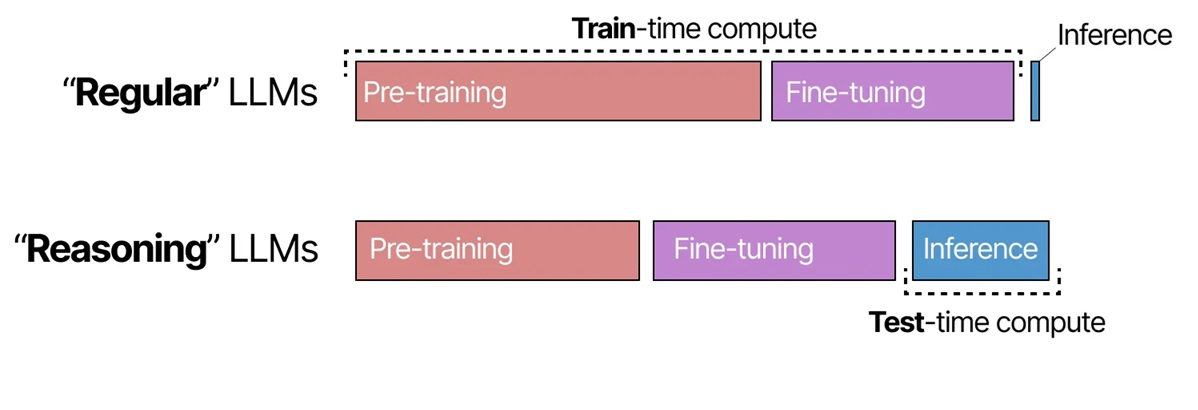
\includegraphics[width=0.8\linewidth,keepaspectratio]{llm212}
		
		{\tiny (Ref: Share of Compute In LLMs - Berto Mill)}
        \end{center}	

\end{frame}

%%%%%%%%%%%%%%%%%%%%%%%%%%%%%%%%%%%%%%%%%%%%%%%%%%%%%%%%%%%
\begin{frame}[fragile]\frametitle{Test Time Compute Example}
\begin{columns}
    \begin{column}[T]{0.5\linewidth}
      \begin{itemize}
        \item Problem: Roger has 5 tennis balls, buys 2 cans with 3 balls each
        \item Regular LLM: Direct answer "11" using 3 tokens
        \item Reasoning LLM: Step-by-step approach using 20 tokens
        \item Step 1: "Roger started with 5 balls" (4 tokens)
        \item Step 2: "Two cans of 3 balls each = 6 balls" (11 tokens)
        \item Step 3: "5 + 6 = 11" (5 tokens)
        \item 6-8x more computational resources but improved accuracy
      \end{itemize}
    \end{column}
    \begin{column}[T]{0.5\linewidth}
        \begin{center}
        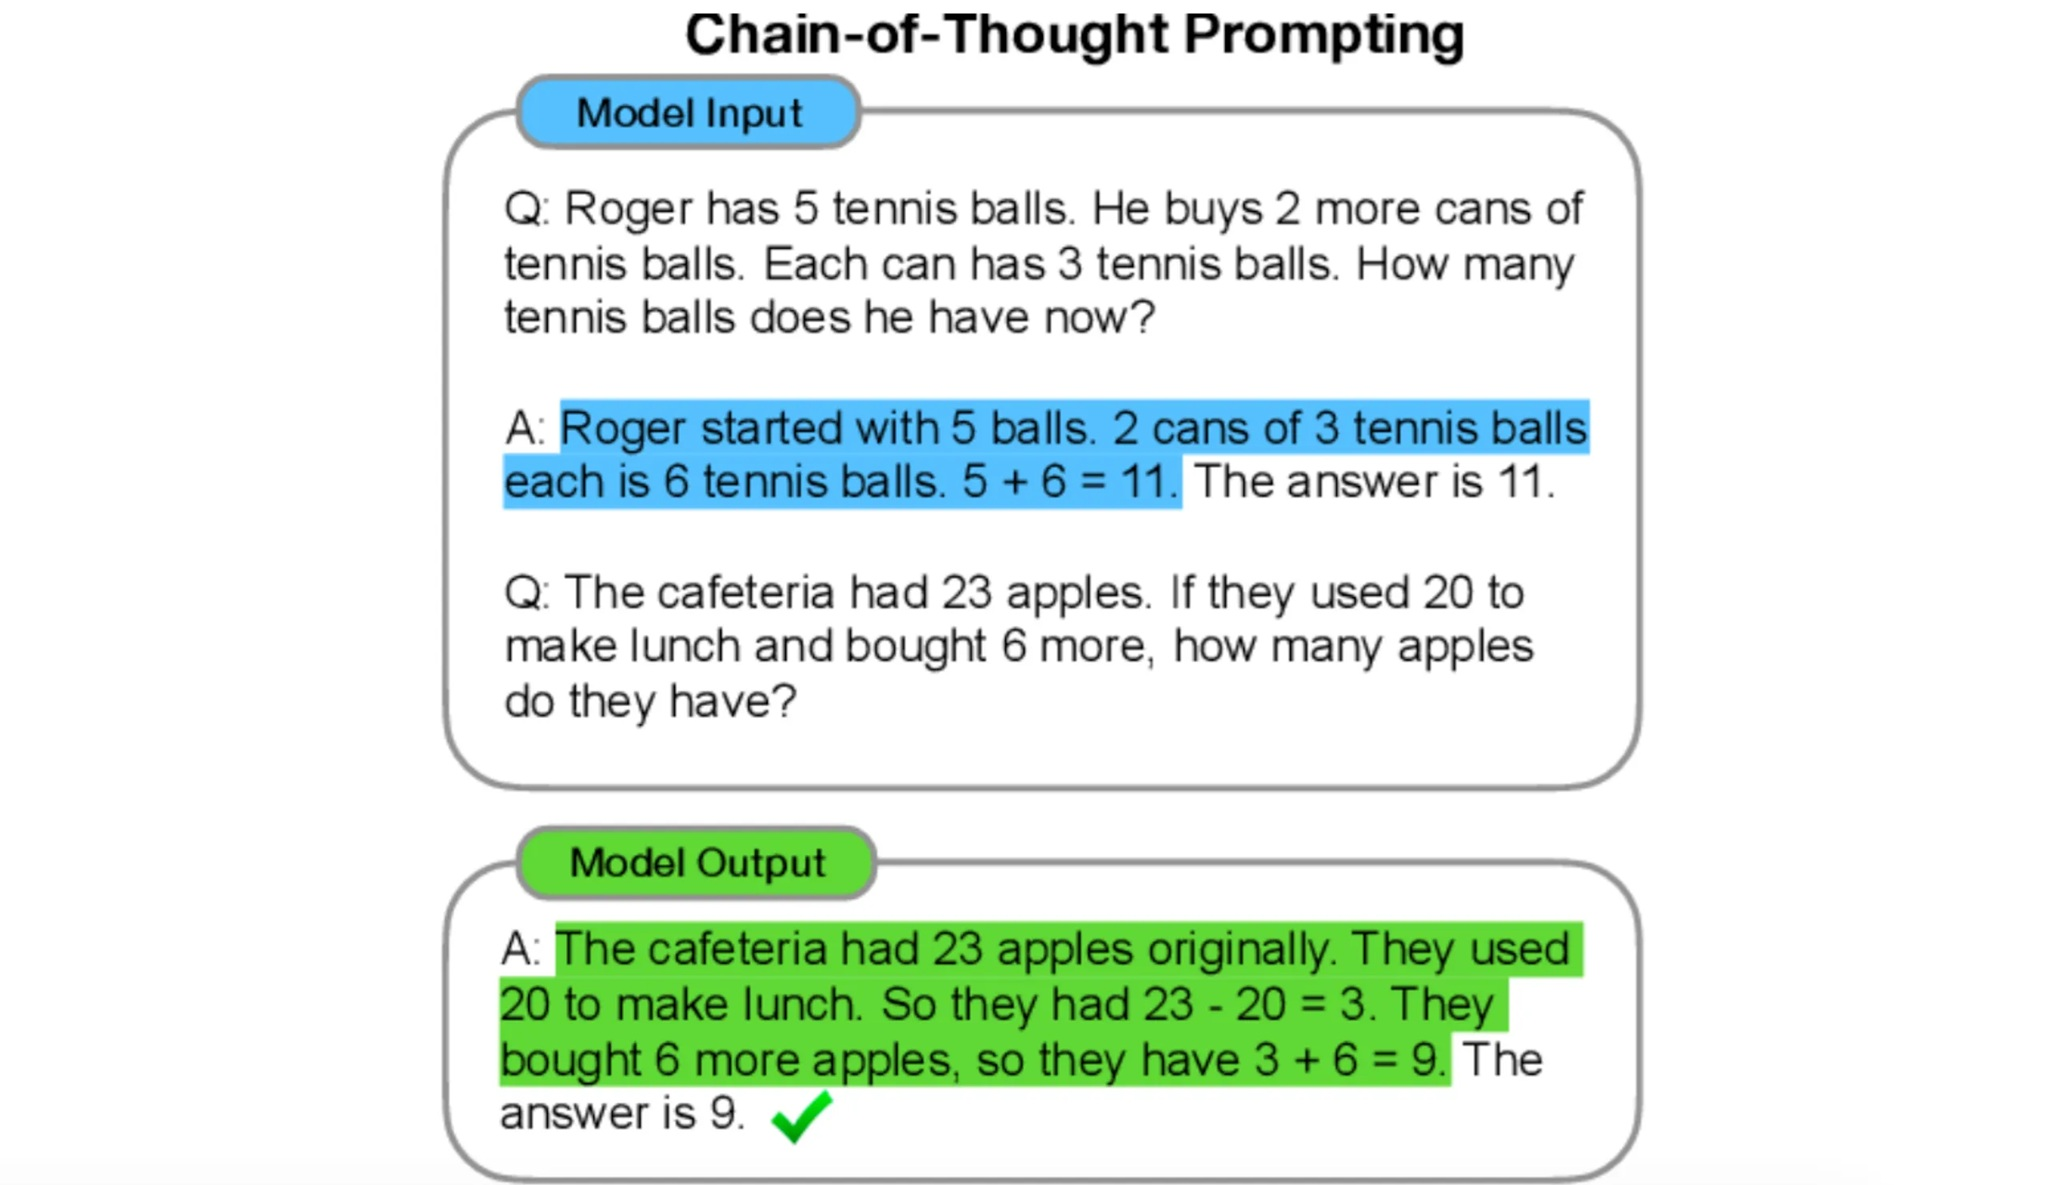
\includegraphics[width=\linewidth,keepaspectratio]{llm213}
		
		{\tiny (Ref: A Brief History of LLMs - LM Pro)}
        \end{center}	
    \end{column}
  \end{columns}
\end{frame}

%%%%%%%%%%%%%%%%%%%%%%%%%%%%%%%%%%%%%%%%%%%%%%%%%%%%%%%%%%%
\begin{frame}[fragile]\frametitle{Chain of Thought Reasoning (2022)}

      \begin{itemize}
	    \item First/simplest way to transform a normal LLM into Reasoning LLM (giving series of steps before outputting the final answer)
        \item Google Brain team's breakthrough paper (12,000+ citations)
			\begin{itemize}
			\item Generating intermediate reasoning steps improves complex reasoning
			\item Arithmetic reasoning benefits from natural language rationales (series of steps)
			\item Simple prompting technique is enough, no model weight changes required
			\item Few-shot prompting with reasoning examples teaches the model
		    \end{itemize}
		
        \item Emergent ability that scales with model size
      \end{itemize}

        \begin{center}
        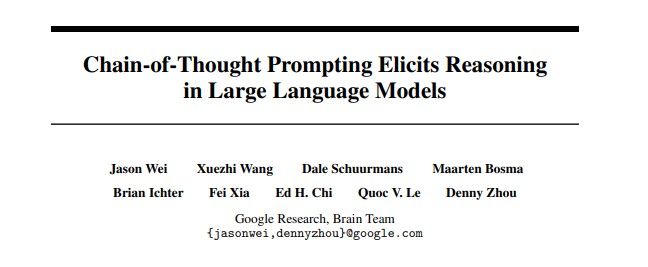
\includegraphics[width=0.8\linewidth,keepaspectratio]{llm214}
		
		{\tiny (Ref: https://arxiv.org/pdf/2201.11903)}
        \end{center}	

\end{frame}

%%%%%%%%%%%%%%%%%%%%%%%%%%%%%%%%%%%%%%%%%%%%%%%%%%%%%%%%%%%
\begin{frame}[fragile]\frametitle{Chain of Thought vs Standard Prompting}

      \begin{itemize}
        \item Standard: Input → Direct Answer
        \item Chain of Thought: Input → Reasoning Steps → Answer
        \item Four linked thoughts forming a reasoning chain
        \item Model learns to apply similar reasoning to new problems
        \item Example: Tennis ball problem broken into logical steps
        \item Demonstrates clear improvement in accuracy and reasoning quality
      \end{itemize}

        \begin{center}
        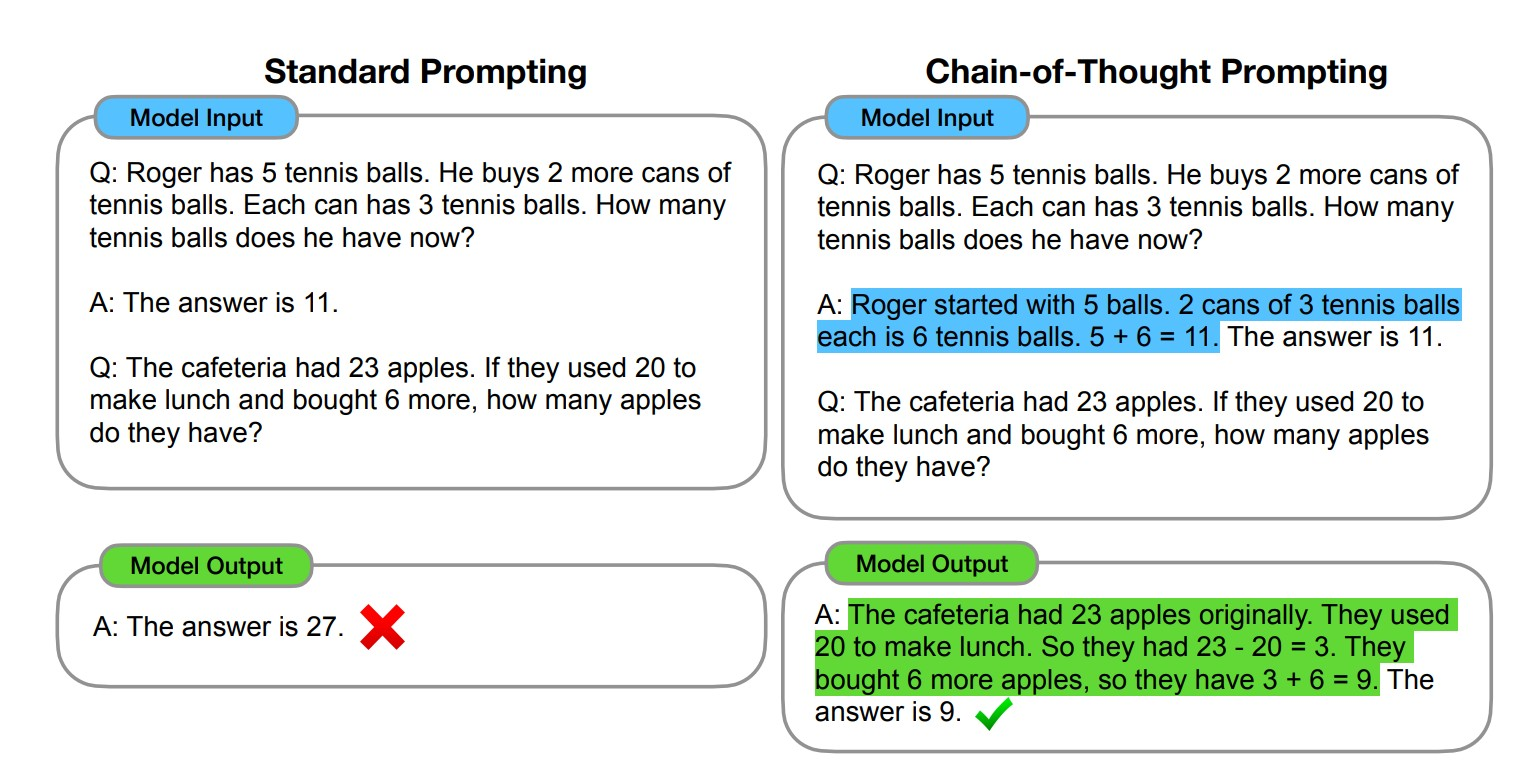
\includegraphics[width=0.8\linewidth,keepaspectratio]{llm215}
		
		{\tiny (Ref: https://arxiv.org/pdf/2201.11903)}
        \end{center}	

\end{frame}

%%%%%%%%%%%%%%%%%%%%%%%%%%%%%%%%%%%%%%%%%%%%%%%%%%%%%%%%%%%
\begin{frame}[fragile]\frametitle{Few-Shot Prompting Foundation}

      \begin{itemize}
        \item Few-shot prompting existed since 2020 (foundational paper)
        \item Provides multiple input-output examples in prompts
        \item Original approach: Direct question → Direct answer
        \item Chain of Thought innovation: Added reasoning steps between input-output
        \item 10-20 demonstration examples guide model behavior
        \item Model learns expected output format and reasoning approach
      \end{itemize}

\end{frame}

%%%%%%%%%%%%%%%%%%%%%%%%%%%%%%%%%%%%%%%%%%%%%%%%%%%%%%%%%%%
\begin{frame}[fragile]\frametitle{Three Types of Reasoning Tasks}
\begin{columns}
    \begin{column}[T]{0.6\linewidth}
      \begin{itemize}
        \item Arithmetic: Mathematical calculations and number problems
        \item Common Sense: "Where might Sammy go to find people?" → Populated areas
        \item Symbolic: Coin flipping logic - heads/tails state tracking
        \item Each requires different Chain of Thought approaches
        \item All three show significant improvement with reasoning prompts
        \item Symbolic reasoning often most challenging for LLMs
      \end{itemize}
    \end{column}
    \begin{column}[T]{0.4\linewidth}
        \begin{center}
        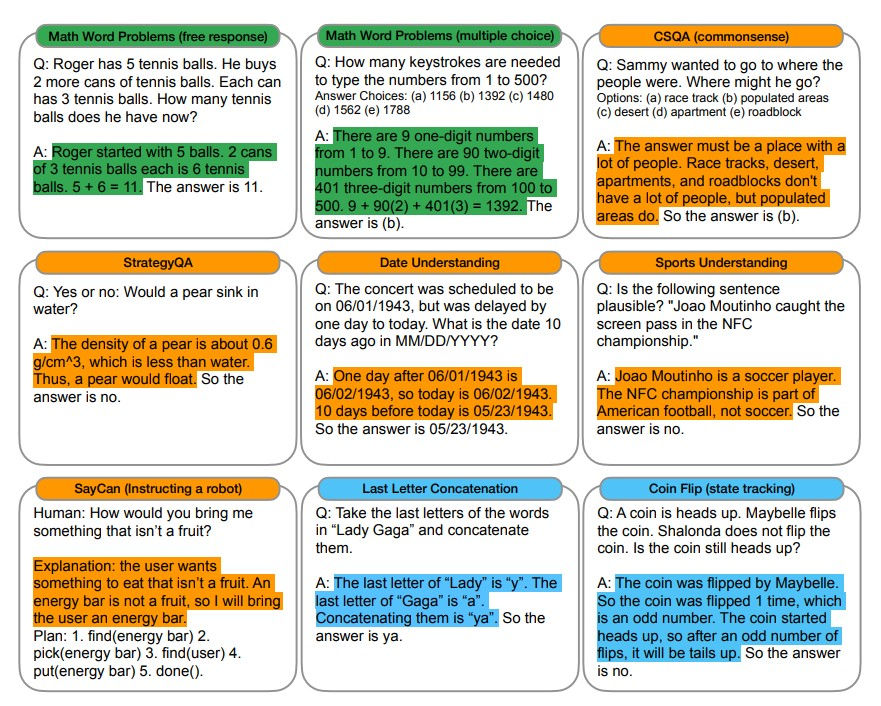
\includegraphics[width=0.8\linewidth,keepaspectratio]{llm216}
		
		{\tiny (Ref: https://arxiv.org/pdf/2201.11903 Examples of (input, chain of thought, output) triples for arithmetic, commonsense, and
symbolic reasoning benchmarks. Chains of thought are highlighted.)}
        \end{center}	
    \end{column}
  \end{columns}
\end{frame}

%%%%%%%%%%%%%%%%%%%%%%%%%%%%%%%%%%%%%%%%%%%%%%%%%%%%%%%%%%%
\begin{frame}[fragile]\frametitle{Model Scale and Reasoning Performance}
\begin{columns}
    \begin{column}[T]{0.6\linewidth}
      \begin{itemize}
        \item PaLM model evaluation on GSM-8K arithmetic dataset
        \item Accuracy increases dramatically with model parameter count
        \item Chain of Thought significantly outperforms standard prompting
        \item Large models (540B params) comparable to supervised fine-tuning
        \item Reasoning is an emergent ability of model scale
        \item Small models fail to understand reasoning nudges effectively
      \end{itemize}
    \end{column}
    \begin{column}[T]{0.4\linewidth}
        \begin{center}
        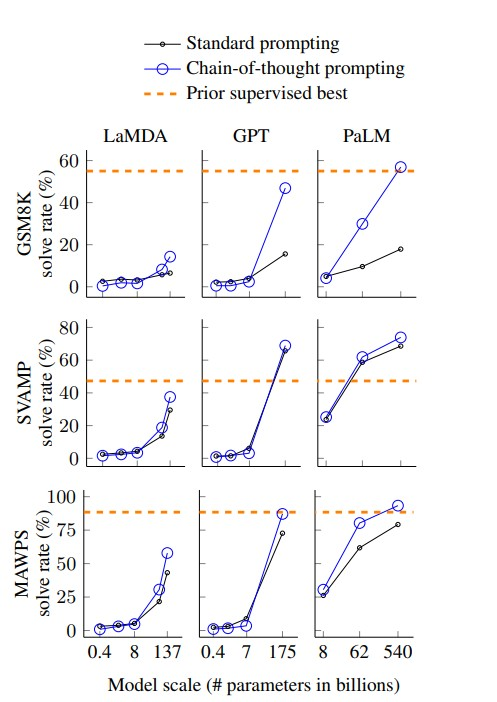
\includegraphics[width=0.8\linewidth,keepaspectratio]{llm217}
		
		{\tiny (Ref: https://arxiv.org/pdf/2201.11903  Chain-of-thought prompting enables
large language models to solve challenging math problems. Notably, chain-of-thought reasoning is an emergent ability of increasing model scale.)}
        \end{center}	
    \end{column}
  \end{columns}
\end{frame}

%%%%%%%%%%%%%%%%%%%%%%%%%%%%%%%%%%%%%%%%%%%%%%%%%%%%%%%%%%%
\begin{frame}[fragile]\frametitle{Zero-Shot Chain of Thought}

      \begin{itemize}
        \item Even simpler approach: "Let's think step by step"
        \item No input-output examples needed (zero-shot)
        \item Single prompt addition triggers reasoning behavior
        \item Two-step process: reasoning generation + answer extraction
        \item Significant performance improvement over plain zero-shot
        \item Works best with sufficiently large models (540B+ parameters)
      \end{itemize}

        \begin{center}
        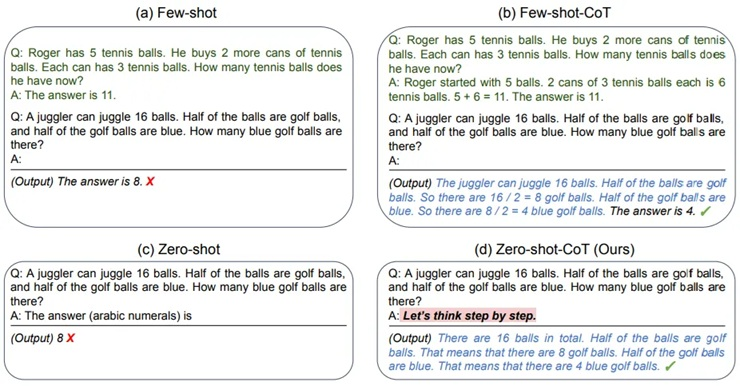
\includegraphics[width=0.8\linewidth,keepaspectratio]{llm218}
		
		{\tiny (Ref: A Brief History of LLMs - LM Pro)}
        \end{center}	

\end{frame}

%%%%%%%%%%%%%%%%%%%%%%%%%%%%%%%%%%%%%%%%%%%%%%%%%%%%%%%%%%%
\begin{frame}[fragile]\frametitle{Practical Implementation Results}

      \begin{itemize}
        \item Tested models: FLAN-T5, TinyLlama, Zephyr (80M-7B parameters)
        \item GSM-8K dataset evaluation with 50 examples
        \item Small models show very low accuracy (0-5\%) - consistent with theory
        \item Models generate reasoning steps but often incorrect final answers
        \item Chain of Thought effective only for very large models
        \item Zero-shot reasoning outperforms few-shot on logical tasks
      \end{itemize}

        \begin{center}
        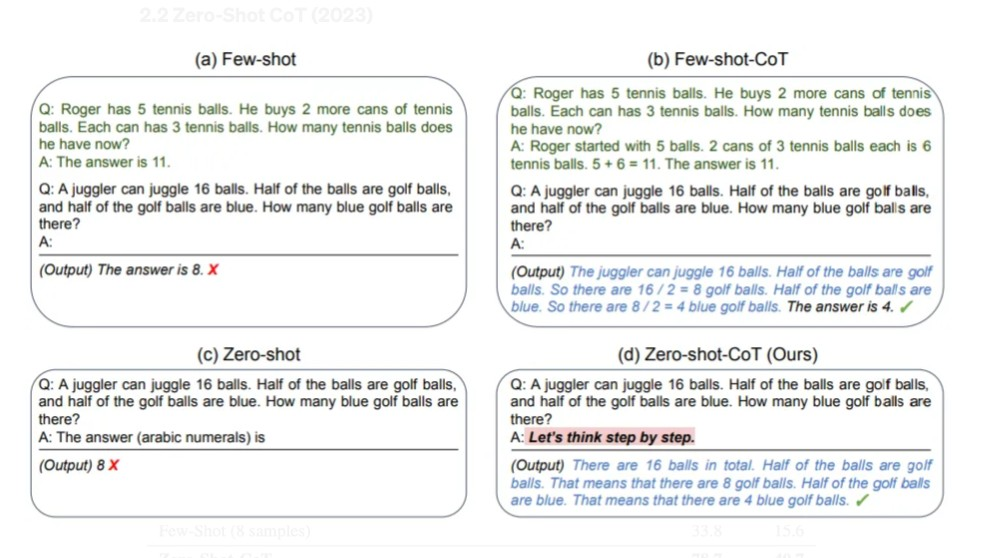
\includegraphics[width=0.75\linewidth,keepaspectratio]{llm219}
		
		{\tiny (Ref: A Brief History of LLMs - LM Pro)}
        \end{center}	

\end{frame}

%%%%%%%%%%%%%%%%%%%%%%%%%%%%%%%%%%%%%%%%%%%%%%%%%%%%%%%%%%%
\begin{frame}[fragile]\frametitle{Key Findings and Implications}

      \begin{itemize}
        \item Reasoning abilities emerge only in sufficiently large models
        \item Test time compute scaling: more thinking = better accuracy
        \item Chain of Thought works across arithmetic, common sense, symbolic tasks
        \item Zero-shot reasoning surprisingly effective with simple prompts
        \item Model size is critical factor for reasoning capability
        \item Future: All major LLM providers developing reasoning models
      \end{itemize}

        \begin{center}
        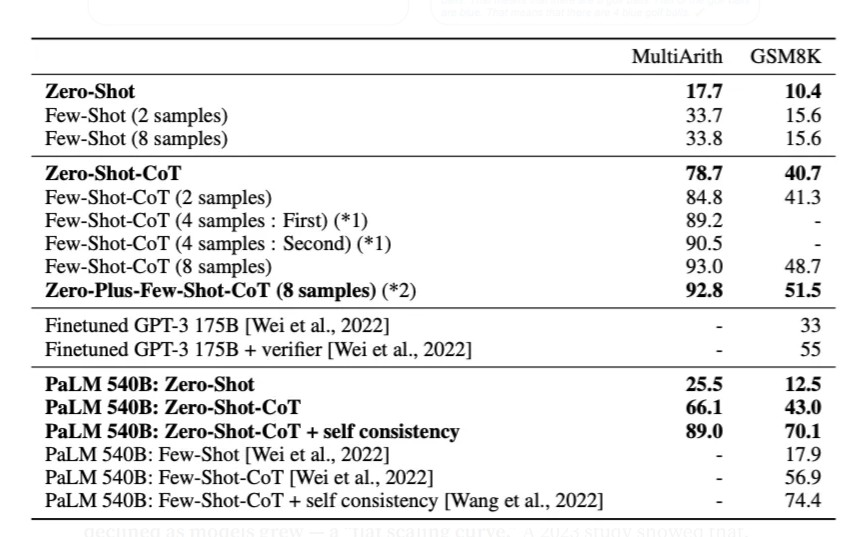
\includegraphics[width=0.7\linewidth,keepaspectratio]{llm220}
		
		{\tiny (Ref: A Brief History of LLMs - LM Pro)}
        \end{center}	

\end{frame}